In the most straightforward form of Shadow Replication, each main is associated with one shadow to tolerate a crash failure, and with two shadows to tolerate a silent failure. 
Similar to traditional process replication, Shadow Replication ensures successful task
completion by running the mains and shadows in parallel. Contrary to process replication, however, Shadow Replication
exploits differential and dynamic execution rates, thereby enabling a
parameterized trade-off between response time, energy consumption and resilience.

After figuring out the shadow suite size according to the fault tolerance requirements, a major challenge resides in determining
jointly the execution rates of all task instances, both before and
after a failure occurs, with the consideration of any objective and any constraint. This chapter addresses the above challenge by formulating it into a generic optimization problem, so that standard and well-known math methods (e.g., quasi-newton) can be naturally applied to solve it and derive the optimal execution rates. With this optimization framework, this chapter also provides a case study in the Cloud with a series of analytical models for failure, power, energy, etc. 

\section{Generic Optimization Framework}
As mentioned in Section~\ref{sec:shadowing_adaptivity}, large-scale computing systems typically aim at maximizing performance, resilience, power/energy consumption, or any of their combination. Given a specific objective, by tuning its execution rates Shadow Replication can be optimized with respect to that objective, while satisfying the provided constraints, if any. A generic optimization framework for this purpose is depicted in Figure~\ref{fig:opt_problem}.

\begin{figure}[t]
	\begin{center}
		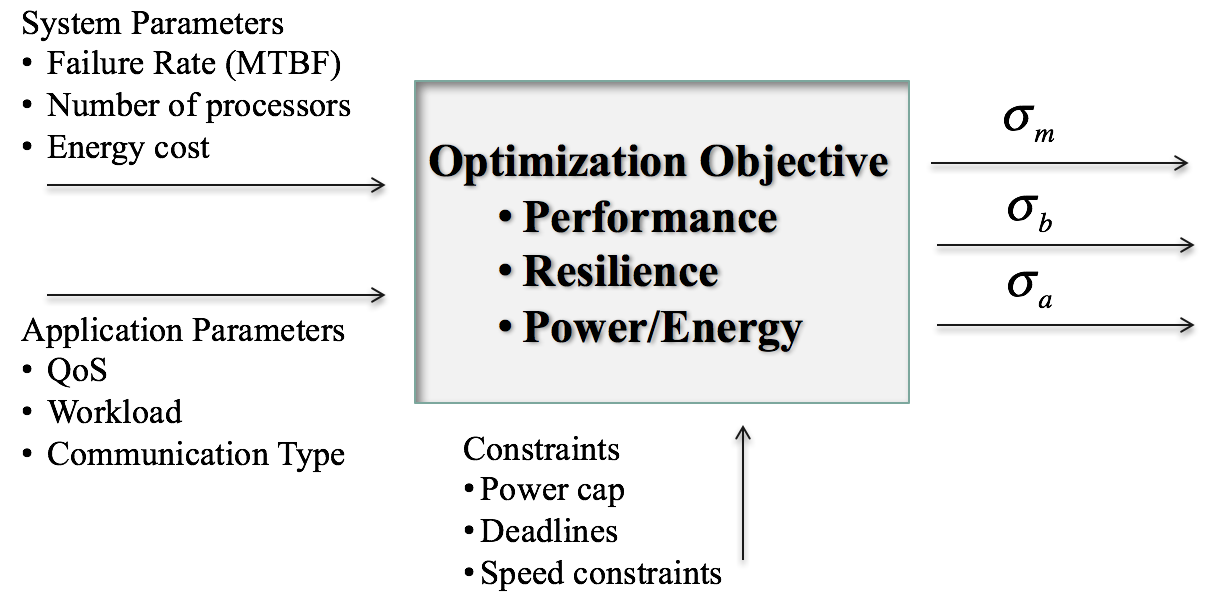
\includegraphics[width=0.9\textwidth]{Figures/opt_problem}
	\end{center}
	\caption{A generic optimization framework for Shadow Replication.}
	\label{fig:opt_problem}
    \vskip -0.1in
\end{figure}

As shown in Figure~\ref{fig:opt_problem}, the inputs to the problem consist of system parameters and application parameters. System parameters include the failure distribution, system scale, and power consumption characteristics. Application parameters could be QoS requirements, total workload, and/or the communication and synchronization patters. In addition, constraints, such as power cap and deadline, can be specified in observation of resource limitations. Finally, the outputs are the derived execution rates for all processes, which optimize the given objective.

The above optimization framework can be tailored to various computing environments for different needs. For example, in HPC systems, the problem can be simplified by fixing $\sigma_m$ and $\sigma_a$ at the maximum CPU rate and only optimize $\sigma_b$ to minimize energy consumption under deadline constraint~\cite{mills_2014_icnc}. The following section discusses another case study in the Cloud environment that relaxes the constraints on $\sigma_m$ and $\sigma_a$~\cite{cui_2014_closer}. The resulting work, referred to as reward-based optimal Shadow Replication, considers Service Level Agreements (SLA) in the Cloud and optimizes a ``reward'' for Cloud service providers. The flexibility in the definition of reward demonstrates the ability of Shadow Replication to achieve objectives that go beyond time and energy. 



\section{Reward-based Optimal Shadow Replication}
Cloud Computing has emerged as an attractive platform for 
diverse compute- and data-intensive applications, as it allows for
low-entry costs, on demand resource provisioning, and
reduced complexity of maintenance~\cite{tchana_cits_2012}. 
As the demand for cloud computing
accelerates, cloud service providers (CSPs) will be faced with the
need to expand their underlying infrastructure to ensure the expected
levels of performance and cost-effectiveness, resulting
in a multi-fold increase in the number of computing, storage and communication components in their data centers.

Two direct implications of the ever-growing large-scale data centers are the increasing energy costs, which build up the operating expenditure, and service failures, which subject the CSP to a loss of revenue. Therefore, Service Level Agreement (SLA) becomes a critical aspect for a sustainable cloud computing business. 
In its basic form, an SLA is a contract between the CSPs and consumers that specifies the terms and conditions under which the service is to be provided, including expected response time and reliability.


To understand the question of how
fault tolerance might impact power consumption and ultimately the expected profit of CSPs, this section studies the application of Shadow Replication to satisfying SLA requirements in the presence of crash failures in Cloud computing. The rest of the section is organized as follows. We begin by describing a parallel computing model typically used in cloud computing for compute- and data-intensive applications. We then present our analytical models and optimization problem formulation, followed by experiments and evaluation. 


\subsection{Cloud Workloads}
Cloud computing workload ranges from business applications and
intelligence, to analytics and social networks mining and log
analysis, to scientific applications in various fields of sciences and
discovery. These applications exhibit different behaviors, in term of
computation requirements and data access patterns. While some
applications are compute-intensive, others involve the processing of
increasingly large amounts of data. The scope and scale of these
applications are such that an instance of a job running one of these
applications requires the sequential execution of multiple computing
phases; each phase consists of thousands, if not millions, of tasks
scheduled to execute in parallel and involves the processing of a very
large amount of data~\cite{lin2010data,Ferdman:2012:CCS:2150976.2150982}. This
model is directly reflective of the \emph{MapReduce} computational
model, which is predominately used in
Cloud Computing \cite{mrbs}.  An instance of this model, is depicted in Figure \ref{fig:map_reduce}.


\begin{figure}[!h]
	\begin{center}
		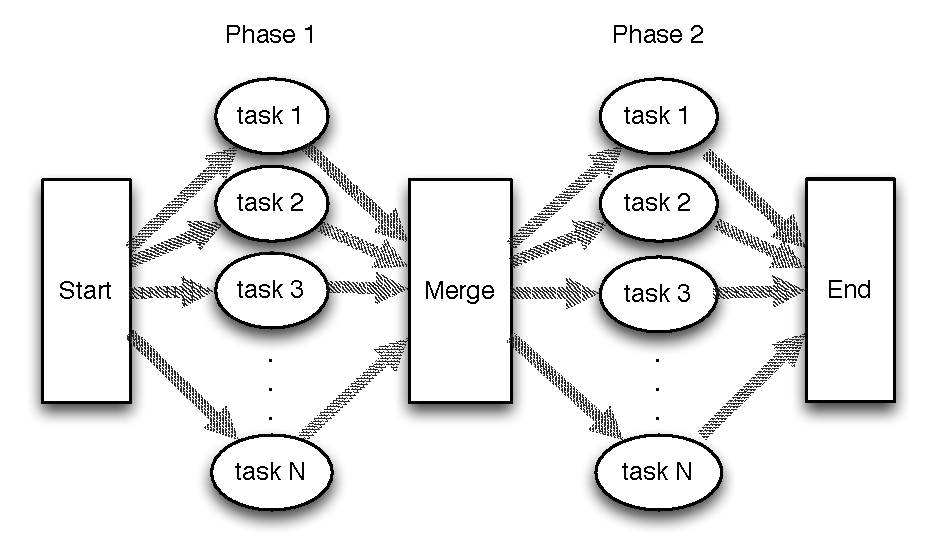
\includegraphics[width=\columnwidth]{Figures/map_reduce.pdf}
	\end{center}
	\caption{Cloud computing execution model with 2 phases.}
	\label{fig:map_reduce}
\end{figure}

Each job has a targeted response time defined
by the terms of the SLA. Further, the SLA defines the amount to be
paid for completing the job by the targeted response time as well as
the penalty to be incurred if the targeted response time is not
met. 

Each task is mapped to one compute core and executes at a rate, $\sigma$. The partition of the job among tasks is
such that each task processes a similar
workload, $W$. Consequently, baring failures, tasks are expected to
complete at about the same time. Therefore, the minimal response time
of each task, when no failure occurs, is
$t_{min}~=~\frac{W}{\sigma_{max}}$, where $\sigma_{max}$ is the maximum execution rate. This is also the minimal response
time of the entire phase. 


\subsection{Optimization}
This part describes an optimization problem for a single job on top of the Cloud computing execution model described above. Using this
framework we compute profit-optimized execution rates for Shadow Replication with dual modular redundancy (i.e., one shadow process per main process): 

\begin{equation}
\label{optimization_problem}
%\setlength{\abovedisplayskip}{14pt}
\begin{alignedat}{2}
\max_{\sigma_m,\sigma_b,\sigma_a}     & E[profit] \\
s.t.                                 & 0 \leq \sigma_m \leq \sigma_{max} \\
                                     & 0 \leq \sigma_b \leq \sigma_{m} \\
                                     & 0 \leq \sigma_a \leq \sigma_{max} 
\end{alignedat}
\end{equation}
We assume that processor execution 
rates are continuous and use nonlinear optimization techniques
to solve the above optimization problem. 

In order to earn profit, service providers must either increase
income or decrease expenditure. We take both factors into
consideration for the purpose of maximizing profit while meeting
customer's expectation. In our model, the expected profit is defined as the expected reward minus the expected expense.

\begin{equation}
E[\text{profit}]=E[\text{reward}]-E[\text{expense}]
\end{equation}

\subsubsection{Reward Model}
\label{sec:sla_reward_model}

The Cloud SLA terms and conditions can be diverse and
complex. To focus on the performance and reliability
aspects of the SLA, we define the reward model based on job completion
time. Platform as a Service (PaaS) companies will continue to become
more popular, causing an increase in SLAs using job completion time as
their performance metric. We are already seeing this appear in
web-based remote procedure calls and data analytic requests.

As depicted in Figure \ref{fig:reward}, customers expect that their
job deployed on Cloud finishes by a mean response time $t_{R_1}$.  As a
return, the service provider earns a certain amount of reward, denoted by R,
for satisfying customer's requirements. However, if the job cannot be
completed by the expected response time, the provider loses a fraction of $R$
proportional to the delay incurred. For large delay, the profit loss may translate into a penalty that the CSP must pay to the customer. In this model, the maximum penalty $P$ is paid if the
delay reaches or exceeds $t_{R_2}$. The four
parameters, $R$, $P$, $t_{R_1}$ and
$t_{R_2}$, completely define the reward model. 
It would be trivial to extend this reward model to any convex function, but we will not bother to do so.

\begin{figure}[t]	
	\begin{center}
		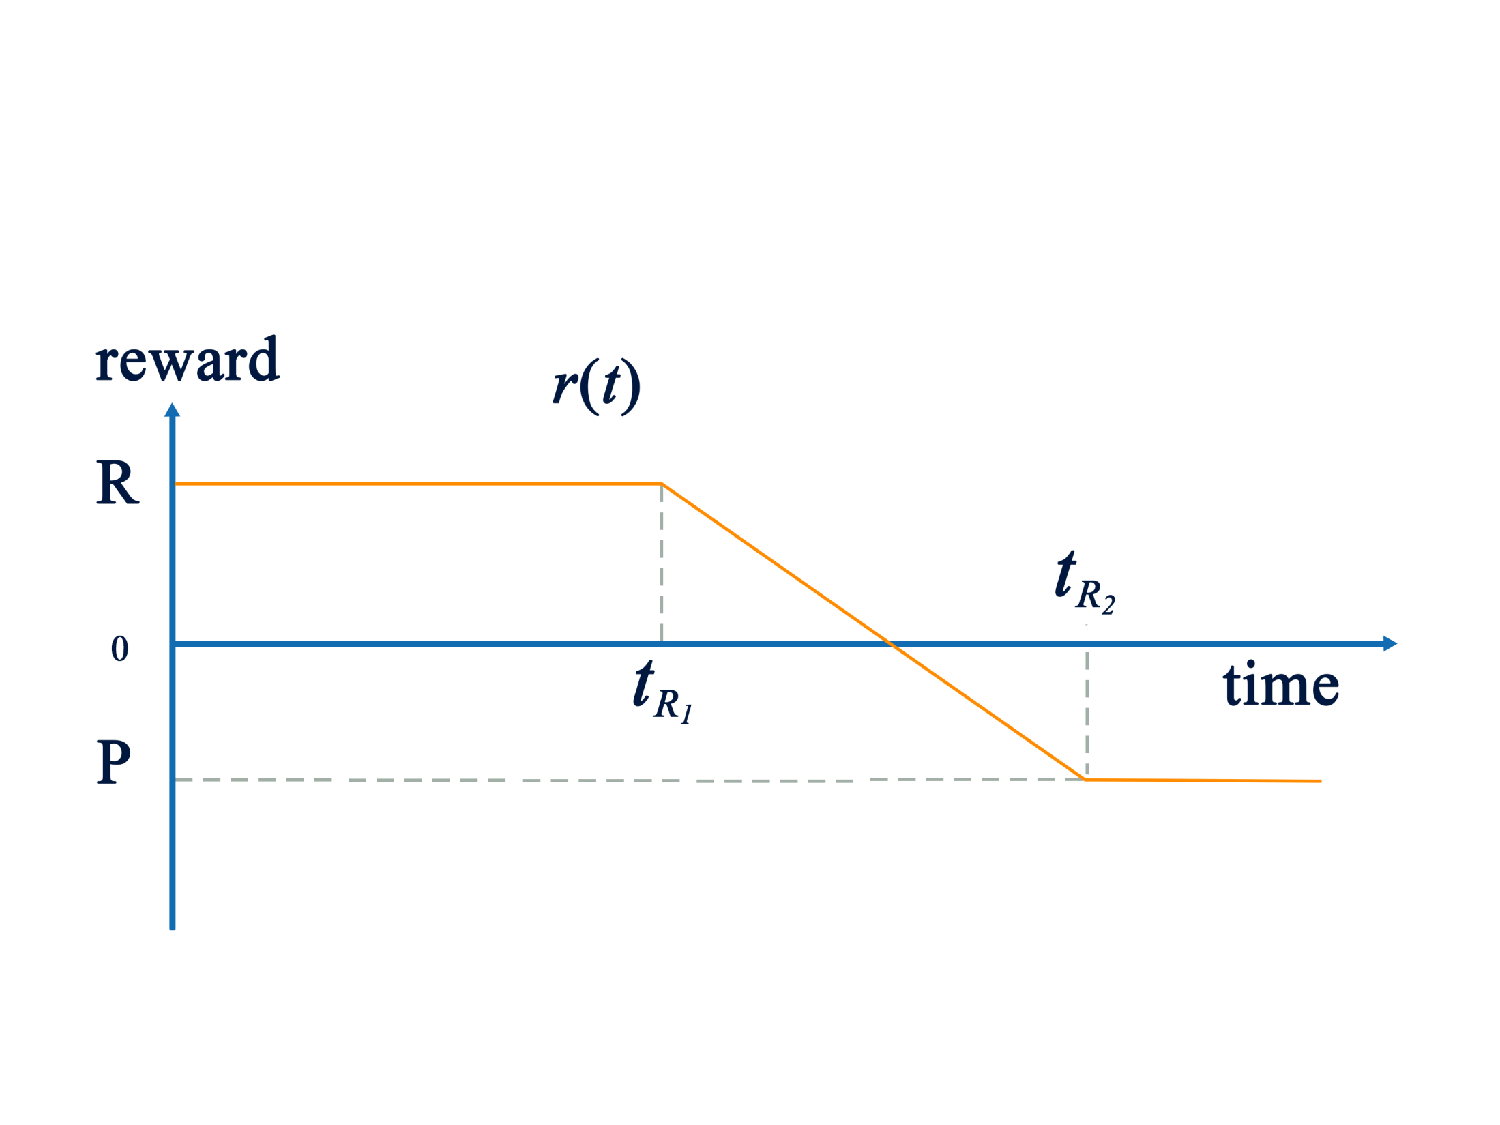
\includegraphics[width=0.8\columnwidth]{Figures/reward.pdf}
	\end{center}
	\caption{A reward model for Cloud computing.}
	\label{fig:reward}
\end{figure}


When applying Shadow Replication with dual modular redundancy to deal with crash failures, 
there are two facts that the service provider must take into account
when negotiating the terms of the SLA. The first is the response time
of the main process assuming no failure (Figure
\ref{fig:sc_no_fail} and Figure \ref{fig:sc_shadow_fail}). This
results in the following completion time:
\begin{equation}
t_c^m=W/\sigma_m
\label{eq:tcm}
\end{equation}

If the main process fails (shown in Figure \ref{fig:sc_main_fail}), the
task completion time by shadow process is the time of the failure,
$t_f$, plus the time necessary to complete the remaining work.

\begin{equation}
t_c^s=t_f+\frac{W-t_f \times \sigma_b}{\sigma_a}
\label{eq:tcs}
\end{equation}

\subsubsection{Failure Model}
Failure can occur at any point during the execution of the main or
shadow process. Our assumption is that at most one failure occurs,
therefore if the main process fails it is implied that the shadow will
complete the task without failure. We can make this assumption because
we know the failure of any one node is rare, thus the failure
of any two specific nodes is very unlikely.

We assume that two probability density functions, $f_m(t_f)$ and
$f_s(t_f)$, exist which express the probabilities of the main and shadow
process failing at time $t_f$, separately. The model does not assume a
specific distribution. However, in the remainder of this section we use
an exponential probability density function, $f_m(t_f)=f_s(t_f)=\lambda
e^{-\lambda t_f}$, of which the mean time between failures (MTBF) is $\frac{1}{\lambda}$.

\subsubsection{Power and Energy Models}
This work assumes DVFS as the underlying execution rate control mechanism. 
DVFS has been widely exploited as a technique to reduce CPU dynamic power~\cite{pillai2001real,flautner2001automatic}. It
is well known that one can reduce the dynamic CPU power consumption at
least quadratically by reducing the execution rate linearly. The
dynamic CPU power consumption of a computing node executing at rate
$\sigma$ is given by the function $p_d(\sigma)=\sigma^n$ where $n \ge 2$.


In addition to the dynamic power, CPU leakage and other components
(memory, disk, network etc.) all contribute to static power
consumption, which is independent of the CPU rate. In this thesis we
define static power as a fixed fraction of the node power consumed
when executing at maximum rate, referred to as $\rho$. Hence, node power consumption is expressed as
$p(\sigma)=\rho \times \sigma_{max}^n + (1-\rho)\times \sigma^n$. When the execution rate is zero
the machine is in a sleep state, powered off or not assigned as a
resource; therefore it will not be consuming any power, static or
dynamic.  Throughout this paper we assume that dynamic power is cubic
in relation to
rate~\cite{rusu2003maximizing,zhai2004theoretical}, therefore the
overall system power when executing at rate $\sigma$ is defined as:
\begin{equation}
p(\sigma) = \begin{cases} \rho \sigma_{max}^3 + (1-\rho) \sigma^3 & \mbox{if } \sigma > 0 \\ 
                          0 & \mbox{if } \sigma = 0 \end{cases}
\label{eq:power_model}
\end{equation}

Using the power model given by Equation~\ref{eq:power_model}, the
energy consumed by a process executing at rate $\sigma$ during an
interval $T$ is given by
\begin{equation}
E(\sigma,T) = p(\sigma) \times T
\end{equation}


Corresponding to Figure~\ref{fig:sc_overview}, there are three cases to consider: main and shadow both succeed, shadow fails, 
and main fails. As described earlier, the case of both the main and
shadow failing is very rare and will be ignored. The expected
energy consumption for a single task is then the weighted average of
the energy consumption in the three cases.

First consider the case where no failure occurs and the main process
successfully completes the task at time $t_c^m$, corresponding to Figure~\ref{fig:sc_no_fail}.
\begin{equation}
E_1 =  ( 1-\int_0^{t_c^m}f_m(t)dt) \times (1 - \int_0^{t_c^m} f_s(t)dt) \times (  E(\sigma_m,t_c^m) + E(\sigma_b,t_c^m))
\label{eq:energy_no_failure}
\end{equation}
The product of the first two factors is the probability of fault-free execution of the main
process and shadow process. Then we multiple this probability by the
energy consumed by the main and the shadow process during this fault
free execution, ending at $t_c^m$.

Next, consider the case where the shadow process fails at some point
before the main process successfully completes the task, corresponding to Figure~\ref{fig:sc_shadow_fail}.
\begin{equation}
E_2 = (1-\int_0^{t_c^m}f_m(t)dt) \times 
      \int_0^{t_c^m}(E(\sigma_m,t_c^m)+E(\sigma_b,t)) \times f_s(t)dt
\label{eq:energy_shadow_fail}
\end{equation}
The first factor is the probability that the main process does not
fail, and the probability of shadow fails is included in the second factor which also contains the energy consumption since it depends on the shadow failure time. Energy consumption comes from the main process until the completion of the task,
and the shadow process before its failure.

The one remaining case to consider is when the main process fails and
the shadow process must continue to process until the task completes,
corresponding to Figure \ref{fig:sc_main_fail}.
\begin{equation}
E_3 = (1-\int_0^{t_c^m}f_s(t)dt) \times \int_0^{t_c^m}(E(\sigma_m,t)+ E(\sigma_b,t)+E(\sigma_a,t_c^s-t))f_m(t)dt
\label{eq:energy_main_fail}
\end{equation}
Similarly, the first factor expresses the probability that the shadow process does
not fail. In this case, the shadow process executes from the beginning to
$t_c^s$ when it completes the task. However, under our ``at most one
failure'' assumption, the period during which shadow process may fail
ends at $t_c^m$, since the only reason why shadow process is still in
execution after $t_c^m$ is that main process has already failed. There
are three parts of energy consumption, including that of main process
before main's failure, that of shadow process before main's failure,
and that of shadow process after main's failure, all of which depend
on the failure occurrence time. 

The three equations above describe the expected energy consumption by a
pair of main and shadow processes for completing a task under
different situations. However, under our system model it might be the
case that those processes that finish early will wait idly and
consume static power if failure delays one task. If it is the case
that processes must wait for all tasks to complete, then this energy
needs to be accounted for in our model. The probability of this is the probability that at least one main process fails,
referred to as the system level failure probability.
\begin{equation}
P_f=1-(1-\int_0^{t_c^m}f_m(t)dt)^N
\label{eq:prob_of_one_main_failure}
\end{equation}
Hence, we have the fourth equation corresponding to the energy consumed  by some processes while waiting in idle. 
\begin{equation}
  \begin{split}
  E_4 = & ( 1-\int_0^{t_c^m}f_m(t)dt) \times (1 - \int_0^{t_c^m} f_s(t)dt) \times  P_f \times 2E(0,t_c^j-t_c^m)  \\ & + \int_0^{t_c^m}f_s(t)dt \times  (1-\int_0^{t_c^m}f_m(t)dt) \times P_f \times E(0,t_c^j-t_c^m) 
  \end{split}
\end{equation}
Corresponding to the first case, neither main process nor shadow
process fails, but both of them have to wait in idle from task
completion time $t_c^m$ to the last task's completion (by a shadow
process) with probability $P_f$. Under the second case, only the main
process has to wait if some other task is delayed since its shadow
process has already failed. These two aspects are accounted in the
first and second lines in $E_4$ separately.  We use the expected
shadow completion time $t_c^j$ as an approximation of the latest task
completion time which is also the job completion time.


By summing these four parts and then multiplying it by $N$ we will have
the expected energy consumed by Shadow Replication for completing a
job of $N$ tasks.
\begin{equation}
E[\text{energy}]=N \times (E_1 + E_2 + E_3 + E_4)
\label{eq:total_energy}
\end{equation}

\subsubsection{Reward and Expense}
Reward is the amount paid by customer for the cloud computing
services that they utilize. It depends on the reward function $r(t)$,
depicted in Figure~\ref{fig:reward}, and the actual job completion
time. Therefore, the income should be either $r(t_c^m)$, if all main
processes can complete without failure, or $r^*(t_c^s)$ otherwise. It
is worth noting that the reward in case of failure should be
calculated based on the last completed task, which we approximate by
calculating the expected time of completion allowing us to derive the
expected reward, i.e. $r^*(t_c^s)=\frac{\int_0^{t_c^m}r(t_c^s) \times
f_m(t)dt}{\int_0^{t_c^m}f_m(t)dt}$. Therefore, the expected reward is approximated by the following equation.
\begin{equation}
E[\text{reward}]= (1-P_f) \times r(t_c^m) + P_f \times r^*(t_c^s)
\end{equation}

%% there is some hand-waving maddness above, unclear how to fix? -bnm

The first part is the reward earned by the main process times the
probability that all main processes would complete tasks without
failure. If at least one main process fails, that task would have to
be completed by a shadow process. As a result, the second part is the
reward earned by shadow process times the system level failure probability.

If $C$ is the charge expressed as dollars per unit of energy consumption
(e.g. kilowatt hour), then the expected expenditure would be $C$ times
the expected energy consumption for all $N$ tasks:
\begin{equation}
E[\text{expense}] = C \times E[\text{energy}]
\label{eq:expense}
\end{equation}

However, the expenditure of running the cloud computing service is more
than just energy, and must includes hardware, maintenance, and human
labor. These costs can be accounted for by amortizing these costs into the
static power factor, $\rho$. Because previous studies have
suggested
that energy will become a dominant factor~\cite{elnozahy2003energy,raghavendra2008no}, we decided to focus on this
challenge and leave other aspects to future work.

\begin{table}[!h]
\caption{Symbols used in reward-based optimal Shadow Replication.}
\centering
\begin{tabular}{|r | c |}
\hline 
Symbols                          & Definition                         \\
\hline \hline
$W$                               & Task workload                    \\
\hline
$N$                               & Number of tasks                 \\
\hline
$r(t)$                          & Reward function       \\
\hline
$R$, $P$                            & Maximum reward and penalty      \\
\hline
$t_{R_1}$, $t_{R_2}$             & Response time thresholds  \\
\hline
$C$                               & Unit price of energy            \\
\hline
$\rho$                          & Static power ratio                 \\
\hline
$t_c^m$, $t_c^s$, $t_c^{j}$                 & Completion time of main, shadow, and the whole job \\
\hline
$f_m()$, $f_s()$                    & Failure density function of main and shadow  \\
\hline
$\lambda$                           & Failure rate    \\
\hline
$P_f$                               & System level failure probability \\
\hline
$\sigma_m$, $\sigma_b$, $ \sigma_a$  & rates of main, shadow before and after failure \\
\hline
\end{tabular}

\label{tbl:symbols}
\end{table}

Based on the above formulation of the optimization problem, the
MATLAB Optimization Toolbox was used to solve the
resulting nonlinear optimization problem. The parameters of this
problem are listed in Table~\ref{tbl:symbols}. 


\section{Profit-aware Stretched Replication}
We compare Shadow Replication to two other replication techniques,
traditional replication and profit-aware stretched replication.
Traditional replication requires that the two processes always execute
at the same rate $\sigma_{max}$. Unlike traditional replication,
Shadow Replication is dependent upon failure detection, enabling the
replica to increase its execution rate upon failure and maintain the
targeted response time, thus maximizing profit. While this is the case
in many computing environments, there are cases where failure
detection may not be possible. To address this limitation, we propose
profit-aware stretched replication, whereby both the main process and
the shadow execute independently at stretched rates to meet the
expected response time, without the need for failure
detection. In profit-aware stretched replication, both the main and
shadow execute at rate $\sigma_r$, derived by optimizing the profit
model.  For both traditional replication and stretched replication,
the task completion time is independent of failure and can be directly
calculated as:
\begin{equation}
t_c=\frac{W}{\sigma_{max}} \text{ or } t_c=\frac{W}{\sigma_r}
\end{equation}

Since all tasks will have the same completion time, the job completion
time would also be $t_c$. Further, the expected income, which depends
on negotiated reward function and job completion time, is independent
of failure:
\begin{equation}
E[reward]=r(t_c)
\end{equation}

Since both traditional replication and profit-aware stretched
replication are special cases of our Shadow Replication paradigm where
$\sigma_m=\sigma_b=\sigma_a=\sigma_{max}$ or
$\sigma_m=\sigma_b=\sigma_a=\sigma_r$ respectively, we can easily derive the
expected energy consumption using Equation~\ref{eq:total_energy} with $E_4$
fixed at 0 and then compute the expected expense using Equation~\ref{eq:expense}.

\section{Re-execution} 
Contrary to replication, re-execution initially assigns a single
process for the execution of a task. If the original task fails, the
process is re-executed. In the Cloud computing execution framework,
this is equivalent to a checkpoint/restart, in which the checkpoint is
implicitly taken at the end of each phase, and because the tasks are
loosely coupled they can restart independently. 

Based on the one failure assumption, two cases must be considered to
calculate the task completion time. If no failure occurs, the task
completion time is:
\begin{equation}
t_c=\frac{W}{\sigma_{max}}
\end{equation}
In case of failure, however, the completion time is equal to the sum
of the time elapsed until failure and the time needed for
re-execution. Again, we use the expected value
$t_f^*=\frac{\int_0^{t_c}t \times f_m(t)dt}{\int_0^{t_c}f_m(t)dt}$ to
approximate the time that successfully completed processes have to
spend waiting for the last one.

Similar to Shadow Replication, the reward for re-execution is the
weighted average of the two cases:
\begin{equation}
E[\text{reward}]=(1-P_f) \times r(t_c) + P_f \times r(t_c+t_f^{*})
\end{equation}

For one task, if no failure occurs then the expected energy can be
calculated as
\begin{equation}
E_5=(1 - \int_0^{t_c} f_m(t)dt) \times (E(\sigma_{max},t_c)+ P_f \times E(0,t_f^{*}))
\label{eq:energy_first_task}
\end{equation}
If failure occurs, however, the expected energy consumption can be calculated as
\begin{equation}
E_6=\int_0^{t_c}(E(\sigma_{max},t) + E(\sigma_{max},t_c)) \times f_m(t) dt
\label{eq:energy_rexecution_task}
\end{equation}
Therefore, the expected energy by re-execution for
completing a job of $N$ tasks is
\begin{equation}
E[energy]=N \times (E_5 + E_6)
\end{equation}

\section{Evaluation}
\noindent This section evaluates the expected profit of each of the fault tolerance
methods discussed above under different system environments. We have identified 5
important parameters which affect the expected profit:
\begin{itemize}
\item Static power ratio $\rho$, which determines the portion of power that is unaffected by the execution rate.
\item SLA - The amount of reward, penalty and the required response times.
\item $N$ - The total number of tasks.
\item MTBF - The reliability of an individual node.
\item Workload - The size, $W$, of each individual task.
\end{itemize}



Without loss of generality, we normalize $\sigma_{max}$ to be 1, so
that all the rates can be expressed as a fraction of maximum
rate. Accordingly, the task workload $W$ is also adjusted such that
it is equal to the amount of time (in hours) required for a single
task, preserving the ratios expressed in
Figure~\ref{eq:tcm} and \ref{eq:tcs}. The price of
energy $C$ is assumed to be 1 unit. We assume that $R$ in our reward model
is linearly proportional to the number of tasks $N$ and the maximum
reward for one task is 3 units, so the total reward for a job is $3
\times N$ units.  However, for the analysis we look
at the average of expenditure and income on each task by dividing the
total expenditure and income by $N$. In our basic configuration we
assume that the static power ratio is 0.5, the task size is 1 hour, the node MTBF 5 is
years, the number of tasks is $100000$, and the response time thresholds for
maximum and minimum rewards are 1.3 hours and 2.6 hours
respectively. Since the maximum power consumption is 1 unit, the
energy needed for the task with one process at maximum rate is also 1
unit. 

\subsection{Sensitivity to Static Power}

With various architectures and organizations, servers deployed at
different data centers will have different characteristics in terms of
power consumption. The static power ratio is used to abstract the
amount of static power consumed versus dynamic power.  

\begin{table}[!h]\small
	\caption{Optimal execution rates for different static power ratio. MTBF=5 years, N=100000, W=1 hour, $t_{R_1}$=1.3 hours, $t_{R_2}$=2.6 hours.}
	\centering
		\begin{tabular}{|p{1cm}|p{1cm}|p{1cm}|p{1cm}|}
		\hline
		$\rho$ & $\sigma_m$ & $\sigma_b$ & $\sigma_a$ \\
		\hline
		0.0 &	0.77 & 	0.65 & 	1.00 \\
		\hline 
		0.1 &	0.78 &	0.66 &	1.00 \\
		\hline
		0.2 &	0.83 &	0.66 &	1.00 \\
		\hline
		0.3	&   0.84 &	0.68 &	1.00 \\
		\hline
		0.4	&   0.85 &	0.70 &	1.00 \\
		\hline
		0.5	&   0.86 &	0.72 &	1.00 \\
		\hline
		0.6	&   0.87 &	0.73 &	1.00 \\
		\hline
		0.7	&	0.91 &	0.81 &	1.00 \\
		\hline
		0.8	& 	1.00 &	1.00 &	1.00 \\
		\hline
		0.9	&	1.00 &	1.00 &	1.00 \\
		\hline
		1.0	&	1.00 &	1.00 &	1.00 \\
		\hline
		\end{tabular}
	\label{tbl:rho}
\end{table}

\begin{figure}[!h]	
	\begin{center}
		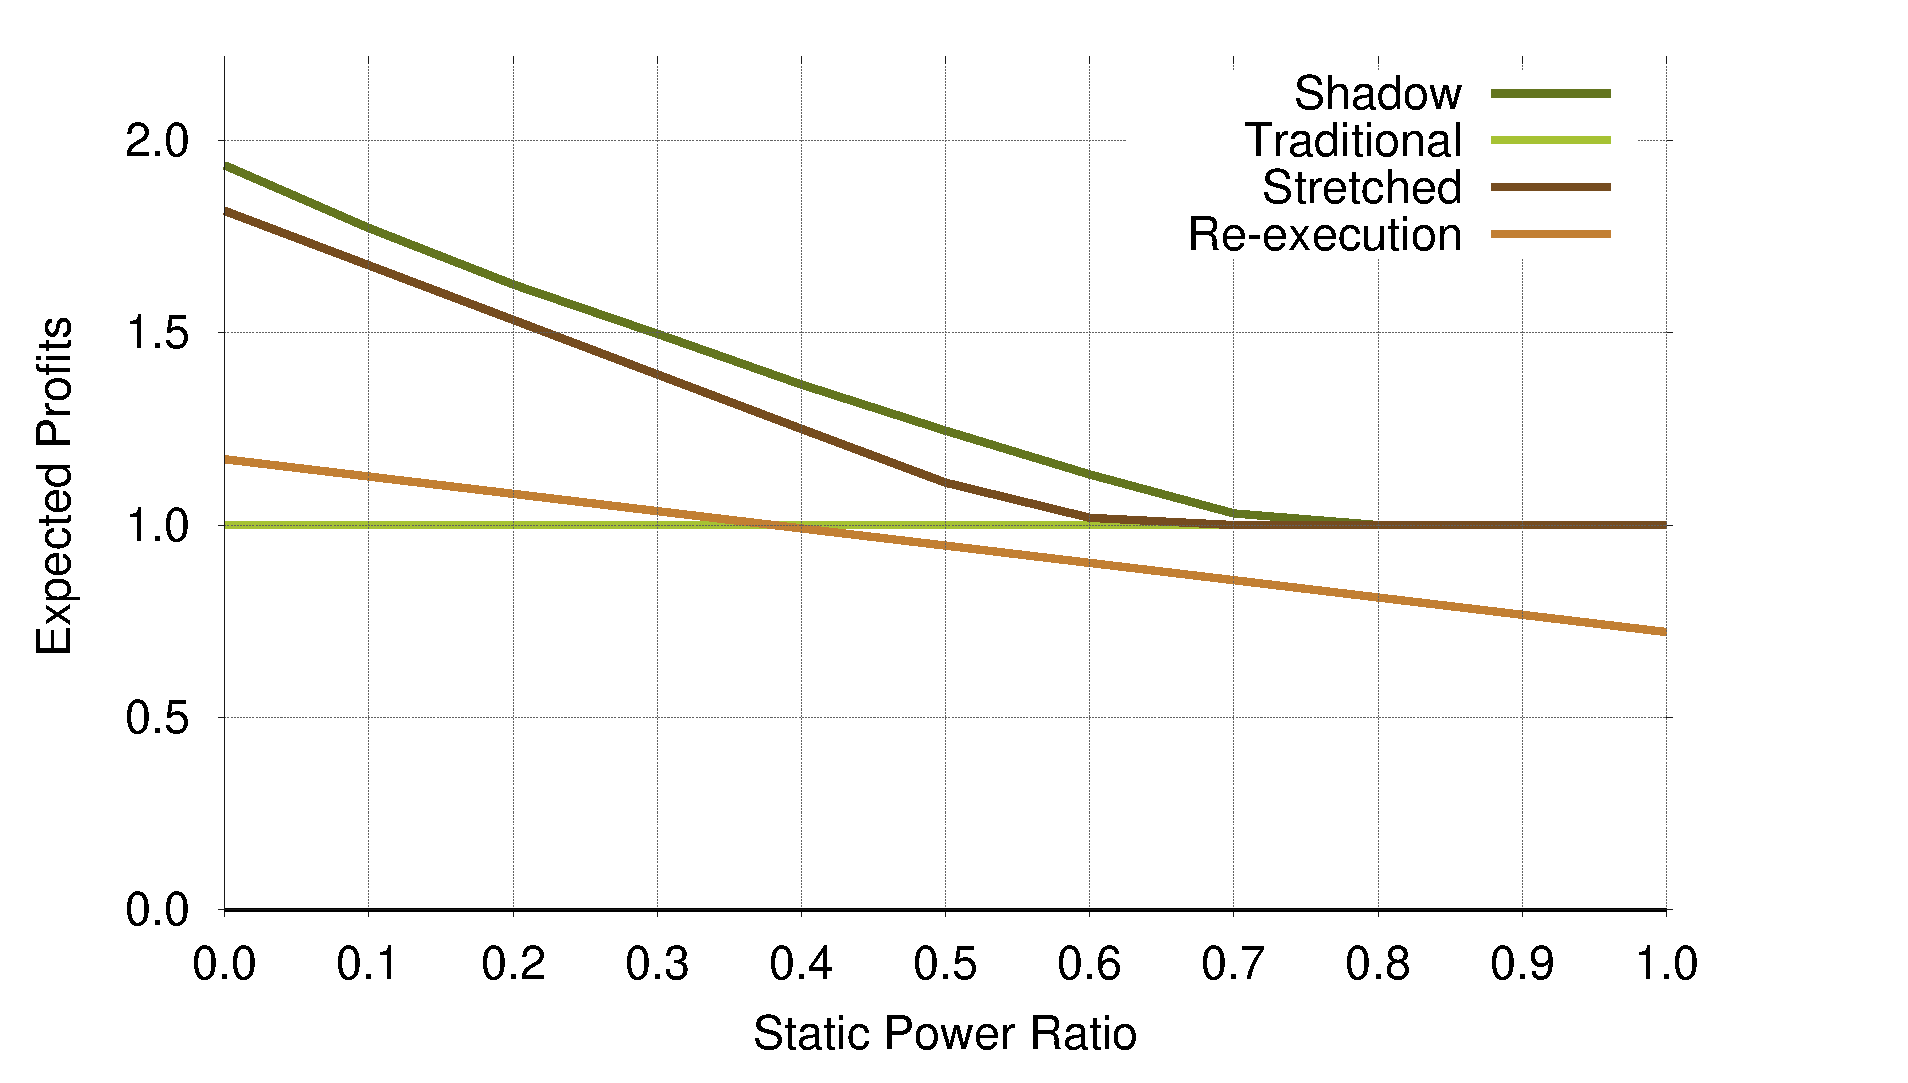
\includegraphics[width=\columnwidth]{Figures/rho_profit}
	\end{center}
	\caption{Profit for different static power ratio. MTBF=5 years, N=100000, W=1 hour, $t_{R_1}$=1.3 hours, $t_{R_2}$=2.6 hours.}
	\label{fig:rho}
\end{figure}

Table \ref{tbl:rho} shows how the profit-optimized execution rates
of Shadow Replication will change as static power increases. The execution rates increase to reduce the execution time as static power ratio increases. Observe
that $\sigma_a$ is always equal to $\sigma_{max}$, which means that after
sensing the failure of the main process, the shadow process should always
shift to maximum rate. This is expected because the optimization will
reduce the amount of work done by the shadow process before failure,
resulting in the maximum execution rate after failure, thus
minimizing the amount of repeated work. 

The potential profit gains achievable by using profit-aware
replication techniques decreases as static power increases, as is shown
in Figure~\ref{fig:rho}. The reason is that our profit-aware
techniques rely upon the fact that one can reduce energy costs by
adjusting the execution rates. Modern systems have a static power between 40\%-70\%~\cite{butts2000static}, and
it is reasonable to suspect that this will continue to be the case in the near future. Within
this target range, Shadow Replication can achieve, on
average, 19.3\% more profit than traditional replication, 8.9\% more
than profit-aware stretched replication, and 28.8\% more than re-execution.


\subsection{Sensitivity to Response Time}

Response time is critical in the negotiation of SLA as customers
always expect their tasks to complete as soon as possible. In this
section we show a sensitivity study with respect to task response
time. We vary the first threshold $t_{R_1}$ from the minimum response
time $t_{min}$ to $1.9t_{min}$, and set the second threshold $t_{R_2}$
to be always $2t_{R_1}$. We do not show results for varying the reward
and penalty values of the SLA. The reason is that changing these
values have no effect on the choice of fault tolerance methods because
they are all affected in a similar way.

\begin{table}[!h]\small
	\caption{Optimal execution rates for different response time threshold. $\rho$=0.5, MTBF=5 years, N=100000, W=1 hour.}
	\centering
		\begin{tabular}{|p{1cm}|  p{1cm}|p{1cm}|p{1cm}|}
		\hline
		$t_{R_1}$ & $\sigma_m$ & $\sigma_b$ & $\sigma_a$ \\
		\hline
		1.0	&	1.00 & 	1.00 &	1.00 \\
		\hline
		1.1	&	0.94 &	0.88 &	1.00 \\
		\hline
		1.2	&	0.89 &	0.79 &	1.00 \\
		\hline
		1.3	&	0.86 &	0.72 &	1.00 \\
		\hline
		1.4	&	1.00 &	0.00 &	1.00 \\
		\hline
		1.5	&	1.00 &	0.00 &	1.00 \\
		\hline
		1.6	&	0.84 &	0.00 &	1.00 \\
		\hline
		1.7	&	0.74 &	0.00 &	1.00 \\
		\hline
		1.8	&	0.64 &	0.00 &	1.00 \\
		\hline
		1.9	&	0.64 &	0.00 &	1.00 \\
		\hline
		\end{tabular}
	\label{tbl:t}
\end{table}

\begin{figure}[!h]	
	\begin{center}
		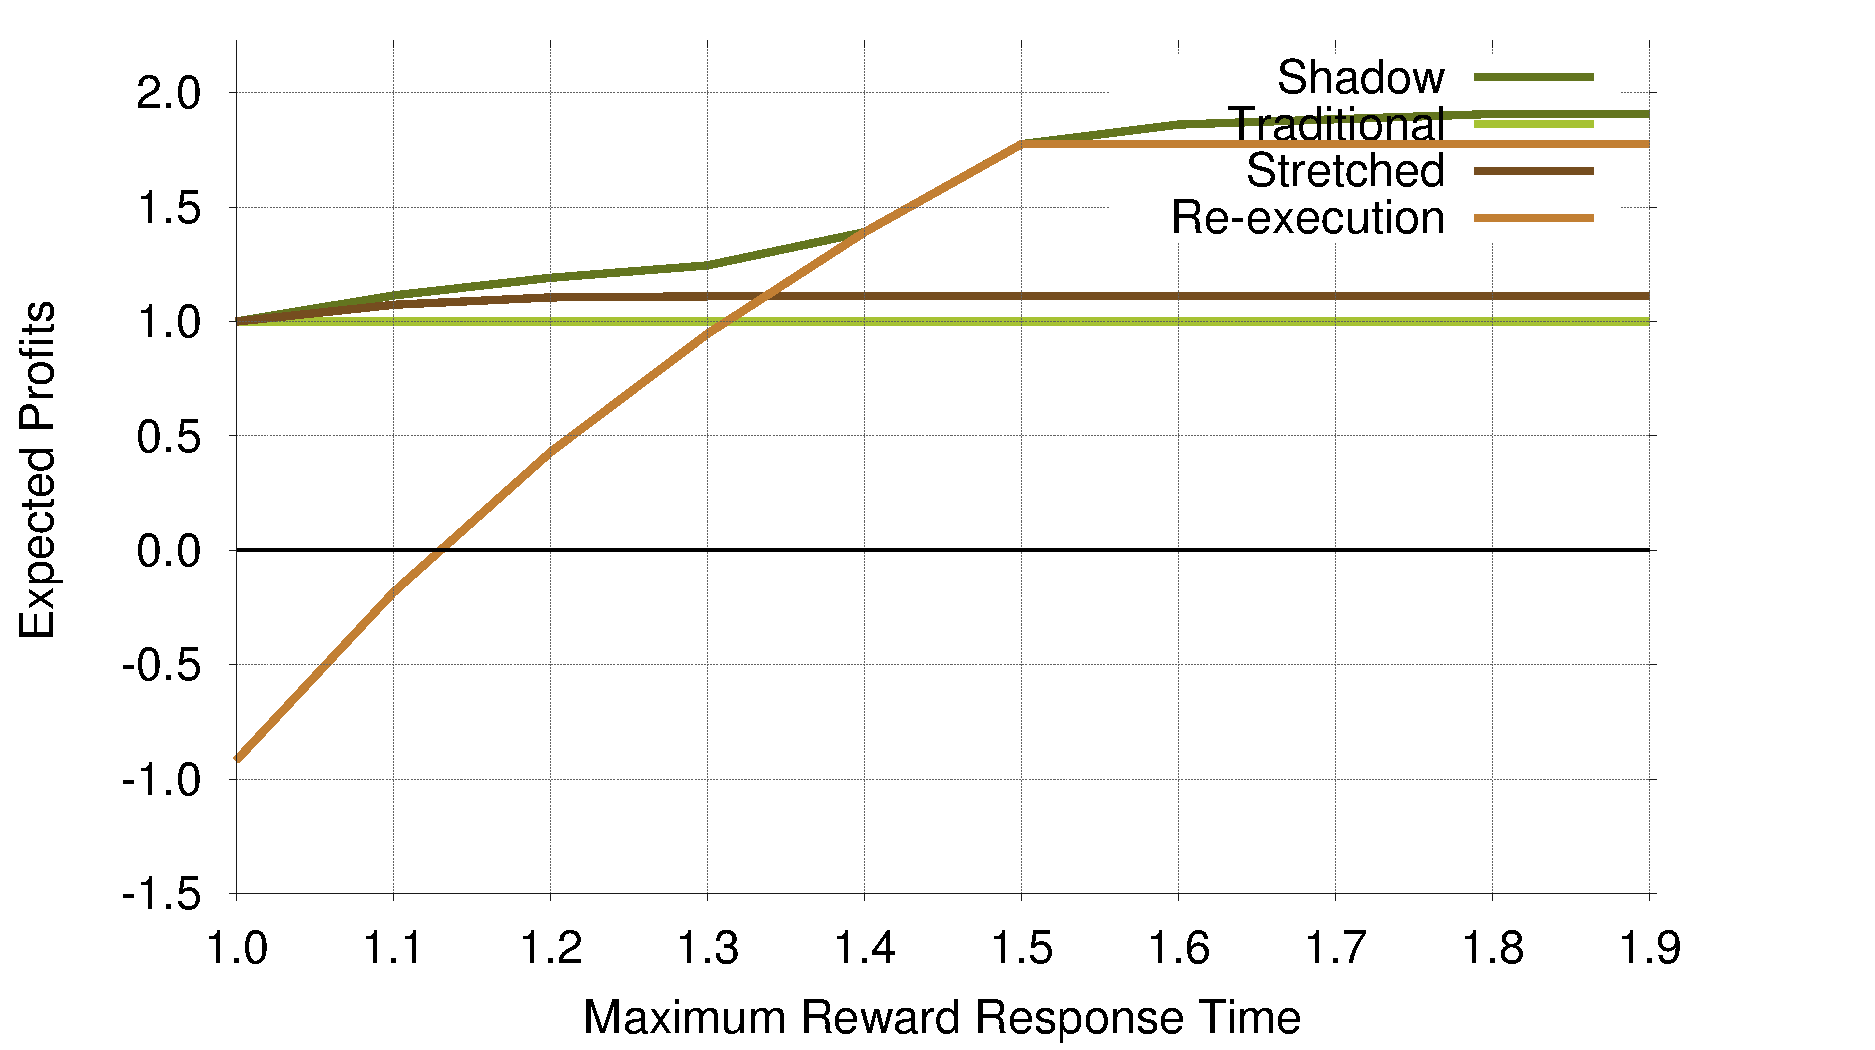
\includegraphics[width=\columnwidth]{Figures/t_profit}
	\end{center}
	\caption{Profit for different response time threshold. $\rho$=0.5, MTBF=5 years, N=100000, W=1 hour.}
	\label{fig:t}
\end{figure}

In Table~\ref{tbl:t} we see that Shadow Replication adapts the execution
rates to take advantage of the available laxity, reducing its rates
as laxity increases. It is clear that Shadow Replication has two different execution strategies separated by $t_{R_1}=1.4$: when time is critical, it uses both a main and a shadow from the very beginning to guarantee that task can be completed on time; when time is not critical, it mimics re-execution and starts its shadow only after a failure.
Also note that as $t_{R_1}$
approaches $t_{min}$, the rates of the main process and the shadow process
converge, effectively causing Shadow Replication to mimic traditional
replication when faced with time-critical jobs.

Figure~\ref{fig:t} shows the effect that targeted response time has upon
the profitability of each fault tolerance method. Compared to traditional replication, all the other methods increase their profit as the targeted
response time increases, this is expected because each of the other
techniques can make use of increased laxity in time to increase
profit. Re-execution is the most sensitive to the target response
time since it fully relies upon time redundancy, showing that it should only be used when the targeted response time is \emph{not} stringent. 
Again, Shadow Replication always achieves more profit than traditional
replication and profit-aware stretched replication, and the profit
gains are 52.8\% and 39.0\% on average. 


\subsection{Sensitivity to Number of Tasks}
The number of tasks has a direct influence upon the system level
failure probability because as the number of tasks increase the
probability that failure will occur to at least one task
increases. Recall that even one failure can hurt the total reward
significantly, and keep the other processes waiting. Thus, Shadow
Replication will adjust its execution rates to reduce the waiting
time.

\begin{table}[!h]\small
	\caption{Optimal execution rates for different number of tasks. $\rho$=0.5, MTBF=5 years, W=1 hour, $t_{R_1}$=1.3 hours, $t_{R_2}$=2.6 hours.}
	\centering
		\begin{tabular}{|r|p{1cm}|p{1cm}|p{1cm}|}
		\hline
		$N$ & $\sigma_m$ & $\sigma_b$ & $\sigma_a$ \\
		\hline
		100			&	0.80	&	0.00	&	1.00 \\
		\hline
		1,000		&	0.84	&	0.00	&	1.00 \\
		\hline
		10,000		&	1.00	&	0.00	&	1.00 \\
		\hline
		100,000		&	0.86	&	0.72	&	1.00 \\
		\hline
		1,000,000		&	0.86	&	0.72	&	1.00 \\
		\hline
		10,000,000	&	0.86	&	0.72	&   1.00 \\
		\hline
		\end{tabular}
	\label{tbl:n}
\end{table}

Table~\ref{tbl:n} is similar to Table~\ref{tbl:t} in that there are also two execution strategies. When there are few parallel tasks, shadow
replication chooses to execute the main processes at nearly full rate and keeps
the shadow processes dormant. The
reason is that it is very likely that all main processes can finish
their tasks successfully, and the need for redundancy is thus less
significant. The other case is when there is a huge number of
tasks to execute, the shadow process would keep running at a slower rate than the main to protect the main as well as save energy. Since the system level failure probability is already 0.9 when $N$ is 100000, the rates stay the same when $N \ge 100000$.

Figure \ref{fig:n} confirms that for small number of tasks
re-execution is more profitable than replication. However, re-execution is not scalable
as its profit decreases rapidly after N reaches 10000. At the same time, traditional
replication and profit-aware stretched replication are not
affected by the number of tasks because neither are affected by the
system level failure rate. On average, Shadow Replication achieves 43.5\%, 59.3\%, and 18.4\%
more profits than profit-aware stretched replication, traditional replication and re-execution, respectively. 

\begin{figure}[!h]	
	\begin{center}
			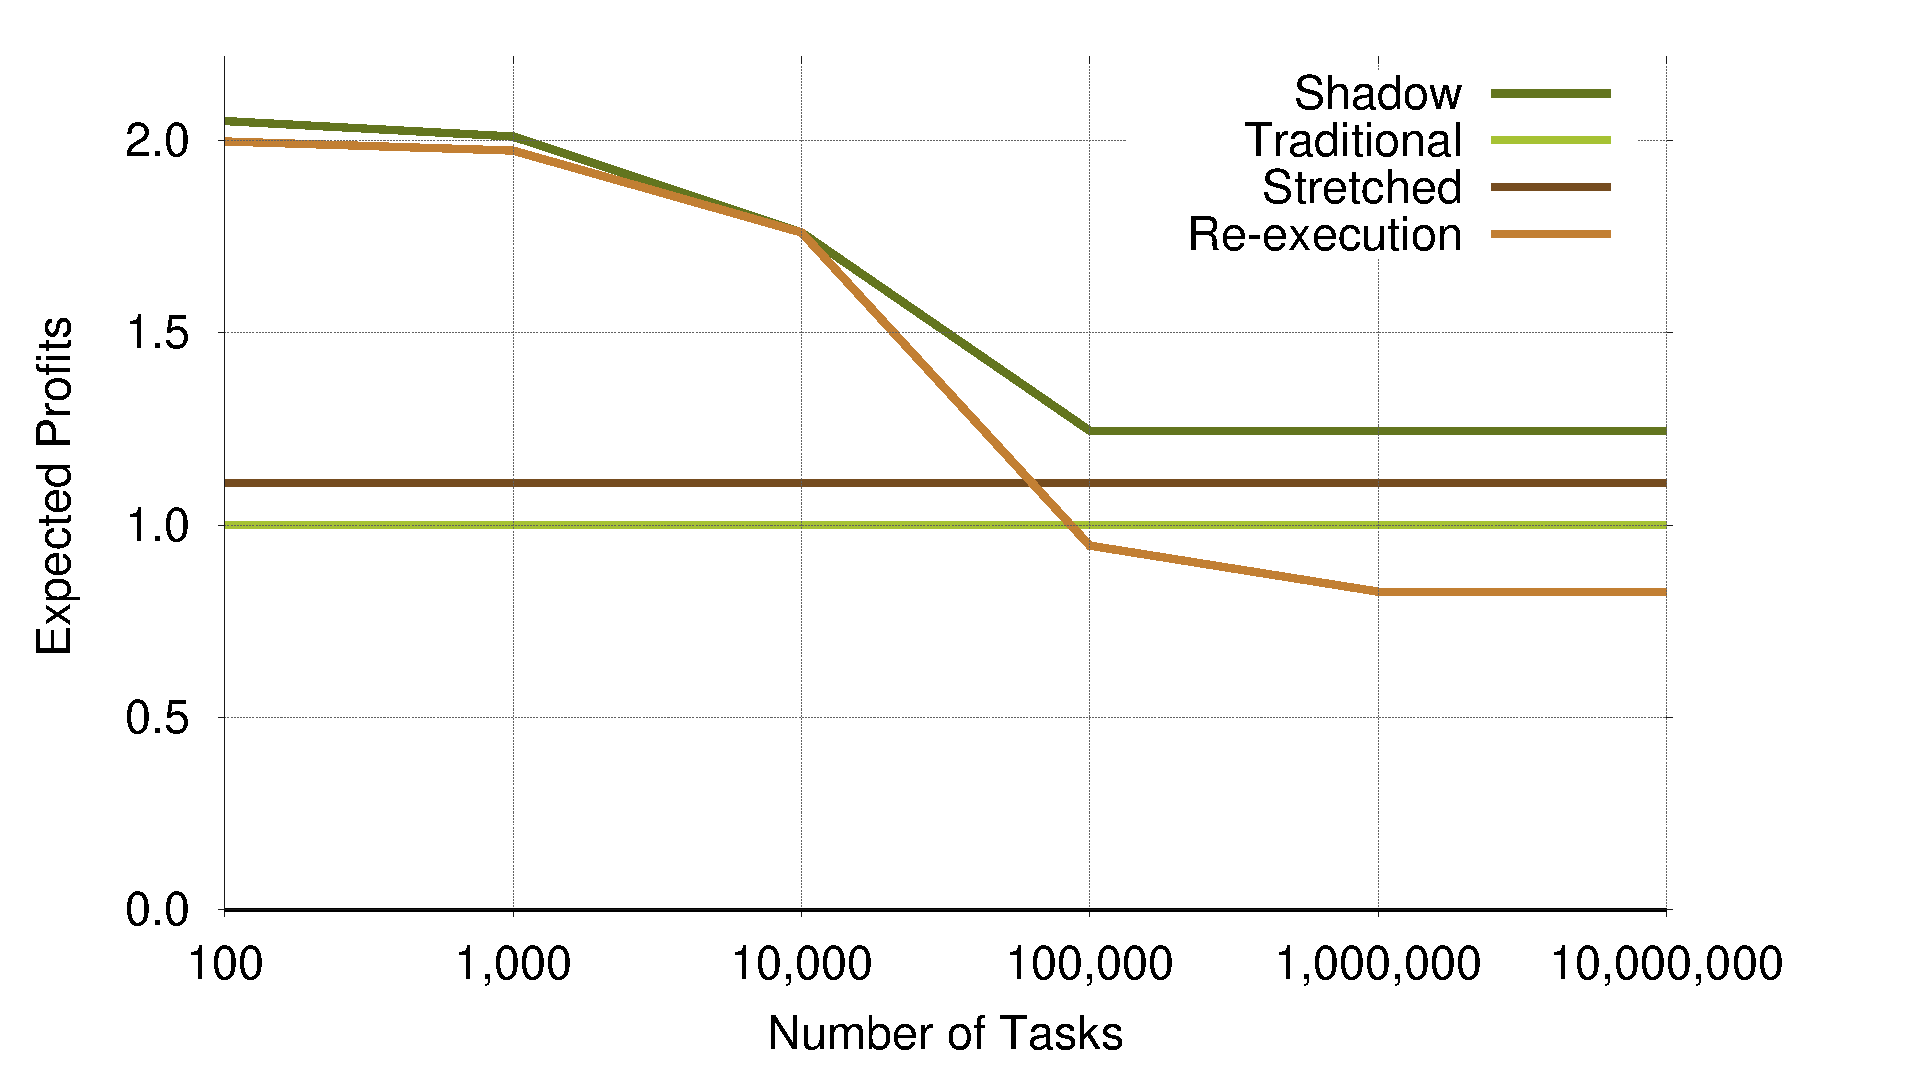
\includegraphics[width=\columnwidth]{Figures/n_profit}
	\end{center}
	\caption{Profit for different number of tasks. $\rho$=0.5, MTBF=5 years, W=1 hour, $t_{R_1}$=1.3 hours, $t_{R_2}$=2.6 hours.}
	\label{fig:n}
\end{figure}

\subsection{Sensitivity to Failure Vulnerability}

The ratio between task size and node MTBF represents the task's
vulnerability to failure. Specifically, it is an approximation of the
probability that failure occurs during the execution of the task. In our
analysis we found that increasing task size will have the same effect
as reducing node MTBF. Therefore, we analyze these together using the
\textit{vulnerability to failure}, allowing us to analyze a wider range of
system parameters.

\begin{table}[!h]\small
	\caption{Optimal execution rates for different task size over MTBF. $\rho$=0.5, N=100000, $t_{R_1}$=1.3 hours, $t_{R_2}$=2.6 hours.}
	\centering
		\begin{tabular}{|c|p{1cm}|p{1cm}|p{1cm}|}
		\hline
		$W/MTBF$ & $\sigma_m$ & $\sigma_b$ & $\sigma_a$ \\
		\hline
		2E-10	&	0.79 &	0.00 &	1.00 \\
		\hline
		2E-09	&	0.79 &	0.00 &	1.00 \\
		\hline
		2E-08	&	0.80 &	0.00 &	1.00 \\
		\hline
		2E-07	&	0.84 &	0.00 &	1.00 \\
		\hline
		2E-06	&	1.00 &	0.00 &	1.00 \\
		\hline
		2E-05	&	0.86 &	0.72 &	1.00 \\
		\hline
		2E-04	&	0.86 &	0.72 &	1.00 \\
		\hline
		2E-03	&	0.86 &	0.72 &	1.00 \\
		\hline
		%2E-02	&	0.86 &	0.72 &	1.00 \\
		%\hline
		\end{tabular}
	\label{tbl:mtbf}
\end{table}

\begin{figure}[!h]	
	\begin{center}
			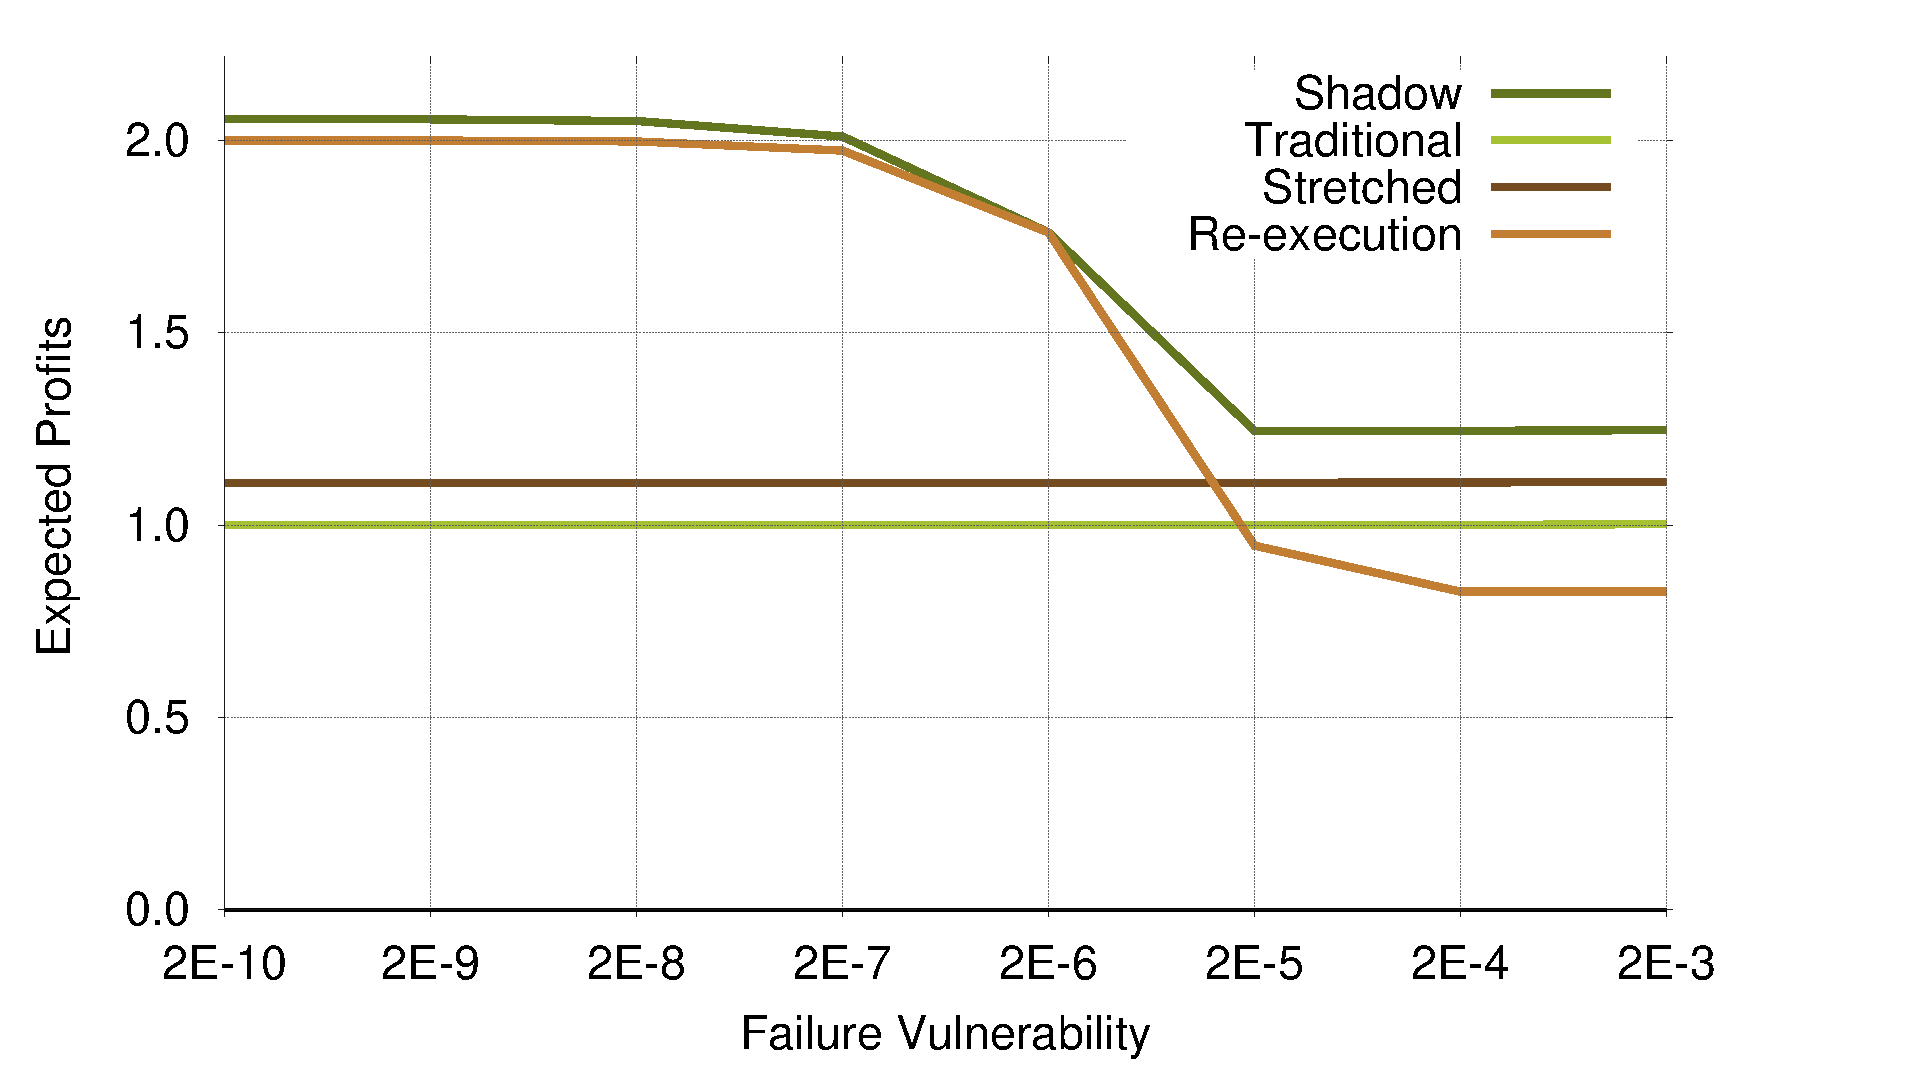
\includegraphics[width=\columnwidth]{Figures/mtbf_profit}
	\end{center}
	\caption{Profit for different task size over MTBF. $\rho$=0.5, N=100000, $t_{R_1}$=1.3 hours, $t_{R_2}$=2.6 hours.}
	\label{fig:mtbf}
\end{figure}

As seen in Table~\ref{tbl:mtbf}, when the vulnerability to
failure is low the execution rates for the shadow process is such
that no work is done before failure. However, as the
vulnerability increases, the shadow process performs more work before
failure. This is analogous to what we observed as we increased the
number of tasks (Table~\ref{tbl:n}). As expected,
re-execution is desired when the vulnerability to failure is
low. As always, Shadow Replication can adjust its execution strategy to maximize the profits, as shown in Figure~\ref{fig:mtbf}.

\subsection{Application Comparison}

To compare the potential benefit of Shadow Replication, we evaluate
the expected profit of each resilience technique using three different
benchmark applications representing a wide range of
Cloud workloads~\cite{mrbs}: Business Intelligence, Bioinformatics and
Recommendation System. The business intelligence benchmark application
is a decision support system for a wholesale supplier. It emphasizes
executing business-oriented ad-hoc queries using Apache Hive. The
bioinformatics application performs DNA sequencing, allowing genome
analysis on a wide range of organisms. The recommendation system is
similar to those typically found in e-commerce sites which, based upon
browsing habits and history, recommends similar
products.

\begin{table}[h]
	\centering
    	\caption{Cloud benchmark applications~\cite{mrbs}.}
		\begin{tabular}{|c|c|}
			\hline
			Application               & Processing Rate \\
			\hline\hline
			Business Intelligence     & 3.3 (MB/s)      \\ \hline
			Bioinformatics            & 6.6 (MB/s)      \\ \hline
			Recommendation System     & 13.2 (MB/s)     \\
			\hline
       \end{tabular}
	   \label{tbl:application_processing_rates}
\end{table}

Using the results of the experiments reported in \cite{mrbs}, we
derived the time required to process data for each application type (Table~\ref{tbl:application_processing_rates}). We assume that
these processing rates per task will not change when scaling the
applications to future cloud environments. This is a reasonable
assumption given that map-reduce tasks are loosely coupled and data
are widely distributed, therefore data and task workload will scale
linearly.

In Figure \ref{fig:app_compare} we compare the expected
profit for each application using each of the 4 resilience techniques. 
We consider two data sizes expected in future
cloud computing environments, 500TB and 2PB. The figure shows that
for business intelligence applications, Shadow Replication achieves significantly larger profits for both data sizes. This
is because business intelligence applications tend to be I/O intensive,
resulting in longer running tasks, whereas recommendation systems tend
to require little I/O, resulting in shorter running tasks, making
re-execution as good as Shadow Replication. Bioinformatics tends to be in between
these two applications, resulting in Shadow Replication performing better
when processing large datasets (2 PB) but not outstanding on smaller
datasets (500 TB). The take-away from this evaluation is that for the
shown system parameters, if phase execution is short, then re-execution
performs as well as Shadow Replication. Alternatively, if a phase is long (20 minutes or
greater), then Shadow Replication can be as much as 47.9\% more
profitable than re-execution. The previous sensitivity analysis can be
used to extrapolate expected profit for different system parameters.


\begin{figure}[!h]
	
	\begin{center}
	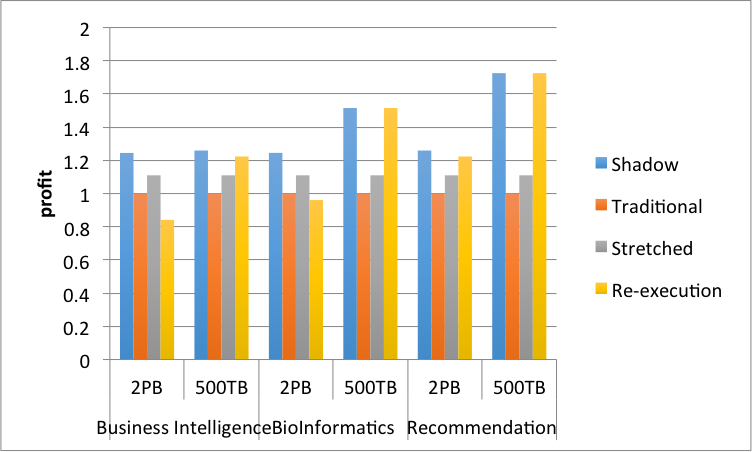
\includegraphics[width=\columnwidth]{Figures/application_comparison.png}
	\end{center}
	\caption{Application comparison. $\rho$=0.5, N=$500000$, $t_{R_1}$=$1.3t_{min}$, $t_{R_2}$=$2.6t_{min}$.}
	\label{fig:app_compare}
\end{figure}





\section{Summary}

In this work we focus on the objective of satisfying SLA in Cloud Computing and demonstrate that Shadow Replication is capable of achieving multi-dimensional QoS goals. 
To assess the performance of the Shadow Replication, an analytical framework is developed and 
an extensive performance evaluation study is carried out. 
In this study, system properties that affect the
profitability of fault tolerance methods, namely failure rate,
targeted response time and static power, are identified. The failure rate is
affected by the number of tasks and vulnerability of the task
to failure. The targeted response time represents the 
clients' desired job completion time.  
Our performance evaluation shows that in all cases, Shadow Replication outperforms
existing fault tolerance methods. Furthermore, Shadow
Replication will converge to traditional replication when target response time is stringent, and to re-execution when target response time is relaxed or failure is unlikely.


   




